\chapter{Optimizing Jastrow Factors for the Transcorrelated Method}
  \label{chap:opt}
\todo{...}

This chapter is based in large part on the following paper:\\
\fullcite{hauptOptimizing2023}

Images have been reused from this paper (with permission).

\section{Introduction}

In this chapter, we investigate the use of flexible Jastrow factors and a novel optimisation strategy for use in \gls{TC} as introduced in section \ref{sec:tc}. As a brief recapitulation, the TC method amounts to a similarity transformation of the Hamiltonian $\hat H$, $\htc = \e^{-J}\hat H\e^J$. However, as this is a non-unitary trasformation, methods used to solve $\htc$ are in general not variational, and hence we are not guaranteed to converge to the \gls{CBS} limit from above. It is therefore important to choose $J$ wisely, as otherwise the method may be highly non-variational, and we may suffer from poor error cancellation.

\todo{...}

\section{Jastrow Factor}

In continuum quantum Monte Carlo methods, the Jastrow factor for a molecule is typically expressed as the sum of electron-electron, electron-nucleus, and electron-electron-nucleus terms,\footnote{Of course, these are not all the possible terms. We may, for example, also choose to include electron-nucleus-nucleus terms.}
\begin{equation}
    \label{eq:jastrow}
    J = \sum_{i<j}^Nv(r_{ij}) + \sum_i^N\sum_I^{N_A}\chi(r_{iI}) + \sum_{i<j}^N\sum_I^{N_A}f(r_{ij}, r_{iI}, r_{jI}),
\end{equation}
where $N_A$ is the number of nuclei, $N$ the number of electrons, and each of $u$, $\chi$, and $f$ are expressed as natural power expansions.\todo{citation} That is,
\begin{equation}
    \label{eq:dtn-jastrow-ee}
    v(r_{ij})    = t(r_{ij},L_v)
                    \sum_{k} a_k r_{ij}^k ,
\end{equation}
\begin{equation}
    \label{eq:dtn-jastrow-en}
    \chi(r_{iI}) = t(r_{iI},L_\chi)
    \sum_{k} b_k r_{iI}^k ,
\end{equation}
\begin{equation}
    \label{eq:dtn-jastrow-een}
    f(r_{ij}, r_{i}, r_{j}) = t(r_{iI},L_f) t(r_{jI},L_f)
    \sum_{k,l,m} c_{klm}
    r_{ij}^k r_{iI}^l r_{jI}^m ,
\end{equation}
where $\{a_k\}$, $\{b_k\}$, and $\{c_{klm}\}$ are linear parameters,
$L_v$, $L_\chi$, and $L_f$ are cut-off lengths, $t(r,L) = (1-r/L)^3
\Theta(r-L)$ is a cut-off function, and $\Theta(r-L)$ is the Heaviside
step function.

As described in chapter \ref{chap:qmc}, \gls{VMC} and \gls{DMC} methods sample electronic configurations $\{\mathbf R\}$ from on a probability distribution based on an analytical trial wave function $\tilde\Psi_{\mathrm T}(\mathbf R)$ to produce a variational estimate of the total energy as an average of the local energy, $E_{\mathrm L}({\mathbf R}) = \tilde\Psi_{\mathrm T}^{-1}({\mathbf R}) \hat H({\mathbf R}) \tilde\Psi_{\mathrm T}({\mathbf R})$ over the sampled configurations.

As described in chapter \ref{chap:explicit}, accurately describing the (electron-electron and electron-nucleus) Kato cusp conditions\supercite{katoEigenfunctionsManyparticleSystems1957a} substationally improves the accuracy of our method. Additionally, in the case of \gls{VMC}, this suppresses extreme outliers in the local energy sampling, allowing meaningful wave function parameters.



% \begin{comment}
%     from paper...

% It is standard practice to apply the electron-electron cusp condition
% on the $u$ term of the Jastrow factor, while the electron-nucleus cusp
% condition is enforced by modifying the $l=0$ component, $\phi(r)$, of
% cuspless molecular orbitals near nuclei so that they exhibit a cusp.
% \cite{Ma_cusp_2005}
% %
% This has been found to be a better approach than applying the
% electron-nucleus cusp condition via the parameters in the $\chi$ term
% of the Jastrow factor. \cite{Drummond_Jastrow_2004, Ma_cusp_2005,
% Needs_casino_2020}

% However, in TC-FCIQMC it is preferable to use unmodified molecular
% orbitals obtained from standard basis sets.
% %
% It would be possible to optimize the Jastrow factor parameters in VMC
% in the presence of cusp-corrected orbitals and use them in TC-FCIQMC
% with a cusp-uncorrected orbital basis, but the Jastrow factor would
% then be sub-optimal by construction in the latter calculation.
% %
% Instead, we recast the cusp-correction scheme of Ref.\
% \onlinecite{Ma_cusp_2005} as an electron-nucleus Jastrow factor term
% $\Lambda$, to be added to (rather than replacing) the $\chi$ term in
% Eq.\ \ref{eq:jastrow}.

% We construct our cusp-correcting Jastrow factor term as
% %
% \begin{equation}\label{eq:cusp-corr-1}
%   \begin{split}
%     \Lambda(r) & = \left[ \ln \tilde \phi(r) - \ln \phi(r) \right]
%                    \Theta(r-r_{\rm c}) \;,
%   \end{split}
% \end{equation}
% %
% where, using the notation of Ref.\ \onlinecite{Ma_cusp_2005}, $r_{\rm
% c}$ is a cut-off radius, $\phi(r)$ is the $l=0$ component of the
% target orbital at the desired nucleus, and $\tilde \phi(r)$ is its
% cusp-corrected counterpart,
% %
% \begin{equation}\label{eq:cusp-corr-2}
%   \tilde \phi(r) = e^{\sum_{l=0}^4 \lambda_l r^l} + C
%                    \quad,\quad r<r_{\rm c} \;.
% \end{equation}
% %
% Here, $\{\lambda_l\}$ are parameters determining the shape of the
% corrected orbital and parameter $C$ is only set to a non-zero value in
% the presence of nodes of $\phi(r)$ near the nucleus.

% Applying continuity and differentiability conditions (see Eq.\ 14 of
% Ref.\ \onlinecite{Ma_cusp_2005}) leaves $\lambda_0$ and $r_{\rm c}$ as
% the only free parameters in Eqs.\ \ref{eq:cusp-corr-1} and
% \ref{eq:cusp-corr-2}.
% %
% Reference \onlinecite{Ma_cusp_2005} describes an approach to obtain
% reasonable values for these parameters, which we use as initial values
% to be refined by the subsequent VMC optimization procedure.
% %
% In practice we evaluate $\phi(r)$ in $\Lambda(r)$ by spline
% interpolation of tabulated data.
% %
% Figure \ref{fig:cusp-term} illustrates the effect of using a $\Lambda$
% term in practice.
% %
% \begin{figure}[!hbt]
%   \begin{center}
%     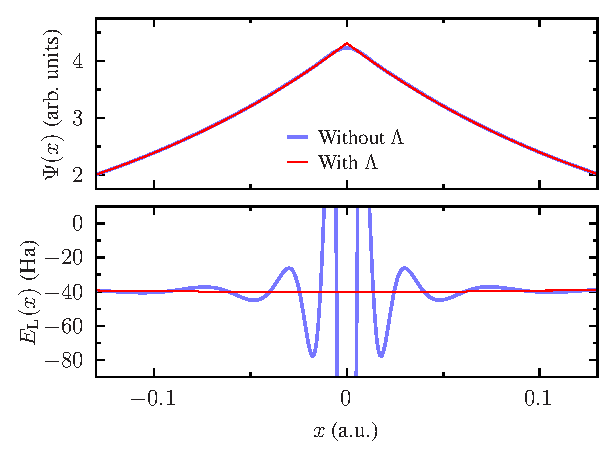
\includegraphics[width=\columnwidth]{Fig/cusp-term}
%     \caption{
%       Wave function value and local energy as a function of the $x$
%       coordinate of an electron in a carbon atom as it crosses the
%       nucleus at $x=0$, both without and with a cusp-correcting
%       $\Lambda$ Jastrow factor term applied to a HF wave function
%       using the cc-pVDZ basis.
%     }
%     \label{fig:cusp-term}
%   \end{center}
% \end{figure}

% For reference, in our calculations we optimize a total of $44$ Jastrow
% factor parameters for the atoms and homonuclear dimers, and $80$
% parameters for the CN dimer; we keep the $L_u$, $L_\chi$, and $L_f$
% cut-off lengths fixed at sensible values for simplicity.
% \end{comment}

\todo{...}

\section{Optimisation Strategy}

We optimise $J$ using \gls{VMC}.

\todo{...}

\subsection{Choosing an Appropriate Sample Size}

\todo{...}

\section{Results}
\todo{mention details about integration will be in a separate chapter}
\todo{mention we use a walker number extrapolation already described in another dissertation (cite Muhammedreza)}
\todo{...}

\subsection{Neglecting Three-Body Excitations}

\todo{...}
\todo{mention Pauli exclusion principle as an argument for why this is a valid approximation (maybe use a figure?)}

\subsection{Basis Set Convergence}

\todo{...}

\section{Conclusion and Outlook}
\todo{mention this is the way we now optimise Jastrow factors, but there is an important extension to the no-3-body approximation, xTC. Briefly describe.}
\todo{...}

\subsection{The xTC Approximation}

\todo{...}

\label{sec:xtc}
